\documentclass[a4paper,11pt]{article}
\usepackage[T1]{fontenc}
\usepackage[utf8]{inputenc}
\usepackage{lmodern}
\usepackage{graphicx}

\title{Principles of Computer System Design\\Assignment 2}
\author{Robert Schmidtke}

\begin{document}

\maketitle

% -----
% -----
% -----
\section{Exercises}
\label{sec:ex}

% -----
\subsection{Serializability \& Locking}
\label{sec:ex1}

\subsubsection*{(a)}
\subsubsection*{(b)}

% -----
\subsection{Optimistic Concurrency Control}
\label{sec:ex2}

% -----
\subsection{Recovery Concepts}
\label{sec:ex3}

\subsubsection*{(a)}
\subsubsection*{(b)}
\subsubsection*{(c)}

% -----
\subsection{ARIES}
\label{sec:ex4}

% -----
% -----
% -----
\section{Programming Task}
\label{sec:pt}

% -----
\subsection{Implementation}
\label{sec:pt1}
The \texttt{Logger} is a singleton that creates a new log file every time it is run or the log is truncated after a checkpoint. It maintains a queue of log requests that gets filled with a new log request on each call of \texttt{logRequest}. Once its thread is started the main loop checks the log queue constantly for new entries. If it finds an entry, it writes it immediately to disk (in the extension (section~\ref{sec:pt5}) it will wait until \(K\) entries are in the queue). If truncation is requested, a new log is started. Similarly, if stopping is requested, the remaining log entries are written to disk and the main loop stops. This procedure serializes log requests that arrive in parallel which realizes overlapping log I/O.

The \texttt{Checkpointer} is a singleton and runs in a separate thread as well. It sleeps for a given timeout and then requests the \texttt{KeyValueBase} to quiesce, then forces all changes to the memory mapped file to disk and truncates the log before resuming the service. Proper quiescing is achieved by every operation acquiring a shared lock before execution and only quiesce acquiring an exclusive lock. This blocks all future operations and waits for all currently running operations to terminate. Resume, on the other hand, releases the exclusive lock, thus allowing for regular operations to resume.

% -----
\subsection{Tests}
\label{sec:pt2}
The logger has been tested excessively by performing all update operations (insert, update, delete and bulkPut), then restarting the server without the memory mapped file being flushed and checking that on startup all changes that have been made are recovered. Additionally the preservation of the init operation has been tested to make sure that the service is already initialized after recovery if it has been previously initialized (and the logger and checkpointer are started accordingly) and, on the other hand, the service will not be initialized after recovery if it has not been initialized before. Naturally these tests take some time which is why only small data sets are used. All test cases are included in the attached source file and the details can be looked up there.

The checkpointer has been tested by performing an update operation, waiting a sufficient amount of time until the checkpointer must have run (and thus flushed the memory mapped file), restarting the server (now with a truncated log) and checking for the previously updated value to still be there. This means that the checkpointer is running very frequently to not make this test take a very long time. Quiescing has been tested manually by artificially delaying the resume operation and sending a couple of update requests to ensure they are only executed after the resume operation has given up the exclusive lock. This test is not included since it contains modification of the service code to ensure the correct behaviour.

% -----
\subsection{Experimental Setup}
\label{sec:pt3}
The performance of the service with logging must be measured against the (otherwise similar) service that does not use logging. Other parameters must remain constant. Therefore the same experiment must be run against these two service implementations. In order to ensure that all other parameters remain fixed, the experiments will be run on the same machine and perform the same sequence of operations on the same data set. Since read operations do not incur log entries, only update operations will be performed. To determine the influence of the number of concurrently operating clients, different sizes of client sets will be used per experiment.

The results will then be averaged over multiple runs. Specifically, the latency per client will be measured as well as the overall time needed to process all requests of all threads, by which the number of requests is then divided to get the throughput. The data set will be keys with just one value to minimize overhead produced by serializing and deserializing, each thread performs 9,000 update requests, so 6 threads perform 45,000 update requests overall.

% -----
\subsection{Experiment}
\label{sec:pt4}
The results of the experiment described in section~\ref{sec:pt3} can be seen in figures~\ref{fig:latency} and~\ref{fig:throughput}.

\begin{figure}[ht]
  \centering
  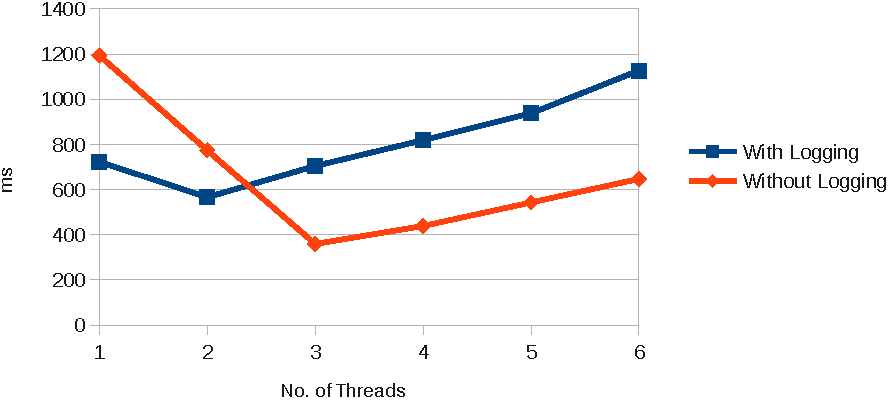
\includegraphics[width=\textwidth]{../experiment/latency-crop-split.pdf}
  \caption{Latency per request/client in nanoseconds}
  \label{fig:latency}
\end{figure}

\begin{figure}[ht]
  \centering
  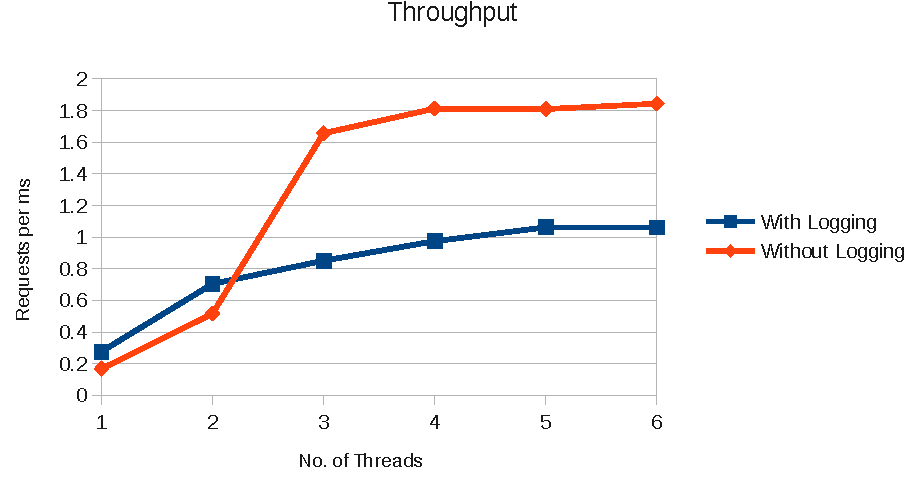
\includegraphics[width=\textwidth]{../experiment/throughput-crop-split.pdf}
  \caption{Throughput as requests per millisecond}
  \label{fig:throughput}  
\end{figure}

The experiment has been carried out using an increasing number of threads where each of them performed the same sequence of 9,000 update operations.

We can see that the latency drops for two threads (which I will use interchangably with 'client') and then slowly increases for each new thread that runs in parallel. The initial drop is expected since for few threads the experiment machine could actually simulate them in parallel, having 4 cores. After that, computing limitations on the machine as well as logging overhead start to kick in giving measures of logging overhead from 74\% to 96\%.

These high values are also due to the fact that the clients and the server ran on the same machine, so there was no network traffic that could dominate the latency. Given the absolute values of fractions of milliseconds it is easy to see that any usage of an intermediate network would affect the latency measured and would definitely decrease the overhead percentage per request. However, given the pure character of the measurements (performed on the same machine without network delays and the only difference between the services being the disabled logging) we can assume that the reported percentage reflects the overhead induced by logging rather accurately.

Similarly, the throughput (requests per millisecond handled by the server) increases but soon reaches a plateau. By the same argument as before, the fact that the logging service can only process from 51\% to 58\% of the requests per millisecond compared to the service without logging illustrates the logging overhead very well.

We can conclude that, on the testing machine used, the overhead induced by logging approaches a constant of about 100\% in latency and a performance decrease of about 50\% in throughput. However, carrying out the experiment with multiple physical clients that do not suffer from being simulated on a limited-core machine as well as requesting the operations via a network would give a more realistic (and less artificial) testing environment.

% -----
\subsection{Extensions}
\label{sec:pt5}
The group commit has been implemented in the logger which waits for a certain amount of log requests to be made before flushing them to disk once or alternatively flushing the queue of accumulated log requests after a certain time has passed since the last flush. The current implementation makes no exceptions for log requests from \texttt{init} for the sake of simplicity. This means that the first call to \texttt{init} blocks all other operations for the amount of time specified in the timeout property. After that the service greatly benefits from multiple clients accessing it in parallel because otherwise the logger would always have to time out before writing logs to disk, thus artificially decreasing the performance. Because of the toy example nature of our implementation, I have mostly tested the commits with \(K=1\) and a timeout of 0, thus practically disabling group commits. However, I have tested manually that operations block until the first init log entry has been written because of a timeout effect. Additionally I have checked that for sufficient parallel requests that exceed \(K\) the log is flushed accordingly.

% -----
% -----
% -----
\section{Notes}
\label{sec:notes}
- unpin, why unpin was not used, no real advantage except memory and this does not count in our small ex, nowhere explained and hashmap also possible\\
- overlapping check

\end{document}
